\section{Analysis Setup}
In this section, we mainly discuss the setup of our analysis. We will introduce the conventions of fixed target collision mode, and the bad run selection from run-by-run QA.
We will also discuss the data sets and the event and track cut we used in this analysis. Finally, the centrality determination will be discussed.
\subsection{Fixed Target Conventions}
In the year 2018, STAR collected fixed-target mode data, the center of mass energy $\sqrt{s_{NN}}$ is 3 GeV (beam energy of 3.85 GeV/u). For the fixed target mode collisions, It is not same as collider mode, the lab frame and the center of mass frame are not same, the midrapidity is not 0. For example, to define the mid-rapidity, we need to boost the measured rapidity in the lab frame into center of mass frame. The midrapidity is half of beam rapidity, beam rapidity can be calculated from this equation.

\begin{figure}
    \centering
    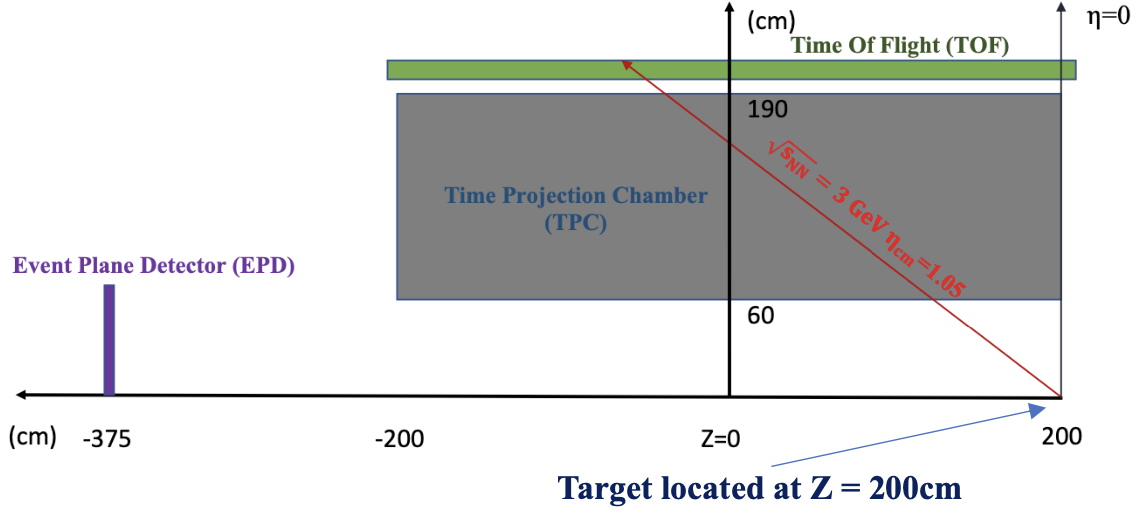
\includegraphics[scale=0.5]{FXT3gev/chapter1/fig/FXT_schematic.jpg}
    \caption{The schematic plot for fixed target collision}
    \label{fig:FXT_schematic}
\end{figure}

\begin{equation}
	y_{b} = cosh^{-1} \left[ \frac{\sqrt{s_{NN}}}{2*m_{p}} \right]
	\label{beamy_cal}
\end{equation}
Where the $\sqrt{s_{NN}}$ is center of mass energy (3 GeV), the $m_{p}$ is proton mass (0.938). In our STAR convention, the beam-going direction is the positive direction (the target is located in the negative rapidity direction $y_{target}$ = -1.045). In order to match the STAR conventions, when calculating rapidity in center of mass frame, in addition to shift by midrapidity, we also need to flip the sign of rapidity. 
\begin{equation}
	y_{CM} = -(y_{lab}-y_{mid})
	\label{rap_convention}
\end{equation}

Figure \ref{fig:FXT_schematic} shows the schematic plot for fixed target collision. In the STAR coordinate system, the target located at Z=200cm the edge of TPC. The EPD located at -375 cm. Red line indicates $\eta$=1.05 and it is roughly midrapidity region.


\subsection{Datasets and Event Selection cuts}
In this study, we analyze the minimum bias events for Au + Au collisions at $\sqrt{s_{NN}}$ = 3 GeV from Fixed target mode, single beam energy is 3.85 GeV. The trigger information and event selection are summarized in the  TABLE \ref{table1}. Since the target is fixed, in our analysis we set the vertex cut along the Z direction is [198, 202] cm, in the X and Y direction, we set the Vr ($\sqrt{Vx^{2}+Vy^{2}}$) less than 2 cm around (0, -2). The total number of minimum bias events is 310 million, and after event cuts (Vz and Vr cut), we still have 280 million good events.

\begin{table}[h]
\centering
\caption{\ Event cuts and total number of minimum bias events}
\label{table1}
\begin{tabular}{l l l l l l l}
%\begin{tabular}
	\hline
\small{\textbf{Energy($\sqrt{s_{NN}}$ GeV)}} & \small{\textbf{Trigger ID (minimum bias)}} & \textbf{Vz(cm)} & \textbf{Vr((0,-2) cm)} & \textbf{Total Events(M))} & \textbf{Good Events(M)}\\
3.0 & 620052 & [198, 202] &2 & 310 & 280 \\
	\hline
\end{tabular}
\end{table}
 
\subsection{Badrun selection}
Due to the detector performance during the data taking, we need to select the bad runs, which might influence our analysis and results. In our analysis, 7 event and track variables (Vz, Vr, refmult, dca, eta, phi, pt) will be used to select bad runs. With event (Vz and Vr) cut,  we plot each variable's mean value as a function of run index in the figure \ref{fig:bad}, totally there are 191 runs at 3GeV. After applying the event cuts (198 $<$ Vz $<$ 202 cm and Vr $<$2 cm), and we plot these variable' mean value as a function of run index, the run index is corresponding to each run number. The second step, we perform minimum and maximum cut (the blue dash line) for each variable to exclude the extreme data(they are far away from the rest of data point). The third step, we calculate the mean value (red solid line) and 3$\sigma$ (red dash line) of the rest data. After that, we can select the bad runs, which are outside the 3$\sigma$ region. totally we have 21 bad runs, these runs will be removed in this analysis.
	

\begin{figure}[ht]
\centering
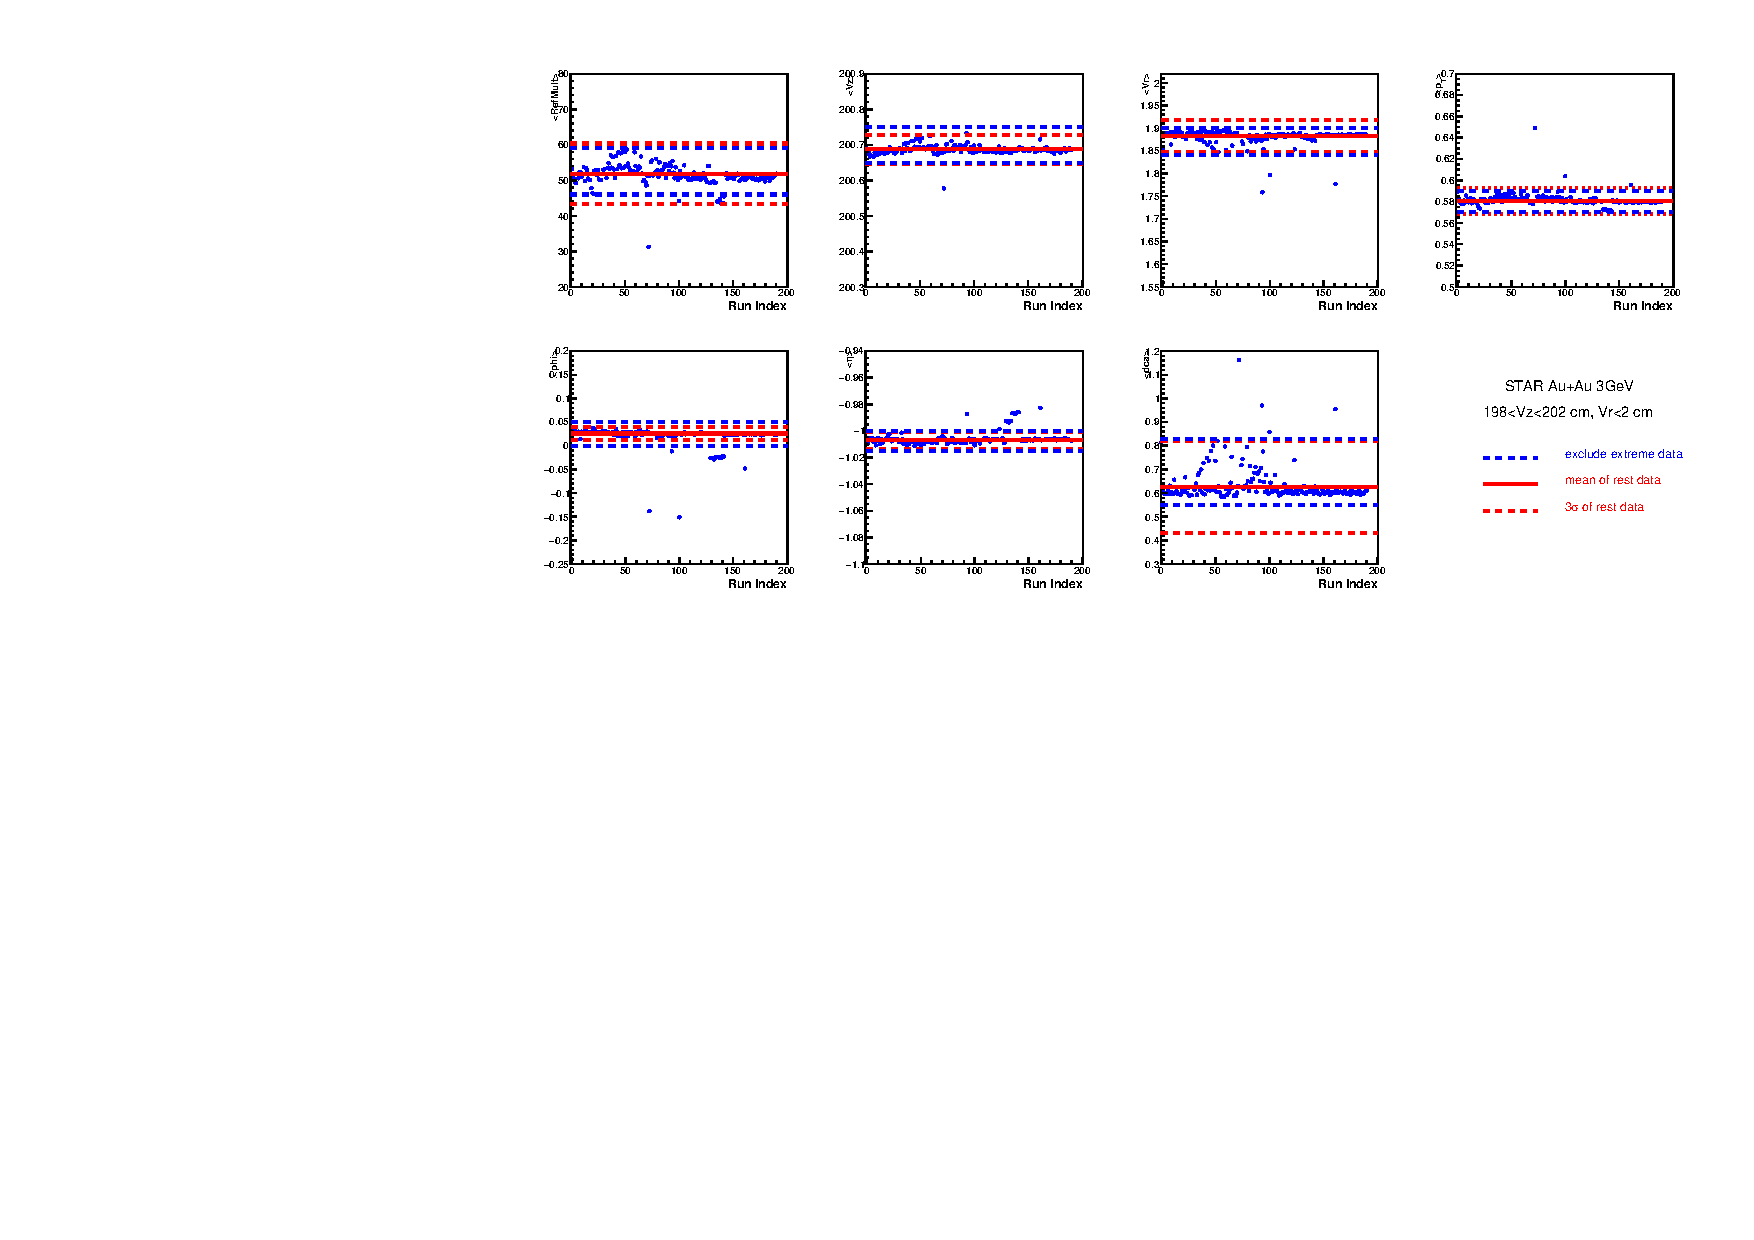
\includegraphics[scale=0.9]{chapter1/fig/badruns.pdf}
\caption{ These variables' (Vz, Vr, refmult, dca, eta, phi, pt) mean value as a function of run index.}
\label{fig:bad}
\end{figure}

From this selection and possible reasons based on shift log in the TABLE \ref{badruns}. The relevant reference could be found at \href{https://drupal.star.bnl.gov/STAR/system/files/Good_run_list_3.85_1.pdf}{Badruns}

\begin{table}[h]
\centering
\caption{\ Bad runs list and what's wrong}
\label{badruns}
\begin{tabular}{cc}
\hline
Bad runs & What's wrong with this run? \\
\hline
\textbf{19151029} & First data run. Fill was with 36 bunches, not 12. \\
\textbf{19152001} & Run has only 1 event.  \\
\textbf{19152078} & 1 minute run, not in the shift log book. \\
\textbf{19153023} & 3.5 minute run, get almost no rate, asked MCR, then TPC trips. \\
\textbf{19153032} & 35 second run, run stopped with TPC trips. \\
\textbf{19153065} & 35 second run, run stopped with two inner TPC trips. \\
\textbf{19154012-19154024} & TPC sector 14 has four RDOs missing. \\
\textbf{19154026} & BTOW is out for this run. \\
\textbf{19154051} & 45 second run, inner TPC tripped during the run. \\
\hline
\end{tabular}
\end{table}


\subsection{Centrality Determination}

Due to the large luminosities at FXT model collisions, more than one collision with the target can happen within the same bunch crossing. It is estimated that there are $\sim$ 1\% of the events and will significantly affect higher moment analyses. In this analysis, the spectator and midrapidity correction is used to consider for pileup events rejection. We can use TPC to measure midrapidity tracks and EPD to measure hits in the forward rapidity region. Detailed information of this method can be found \href{https://drupal.star.bnl.gov/STAR/system/files/PileupFXT3GeV_BulkCorr.pdf}{pileupremove}.

For the centrality definition, we start from uncorrected multiplicity distribution for charged tracks. In order to simulate this distribution, firstly the simulated multiplicity density is calculated using the two component model \cite{Kharzeev:2000ph} with the number of participants $N_{part}$ and number of collision $N_{coll}$ extracted from the Glauber Monte Carlo simulation as formula \ref{equ:two_com}.

\begin{equation}
    \frac{dN_{ch}}{d\eta} = n_{pp} \left [(1-x)\frac{N_{part}}{2} +xN_{coll}\right]
    \label{equ:two_com}
\end{equation}

where the $n_{pp}$ is average multiplicity in minimum-bias p+p collisions and x is the fraction of the hard component. The event-by-event multiplicity fluctuation has been taken into account by convoluting the negative binomial distribution (NBDs) for a given $N_{part}$ and $N_{coll}$. The NBD distribution in multiplicity n has two parameters, $n_{pp}$ and k, and is defined as formula 

\begin{equation}
    P_{NBD}(n_{pp},k;n) = \frac{\Gamma(n+k)}{\Gamma(n+1)\Gamma(k)} \frac{(n_{pp}/k)^{n}}{(n_{pp}/k+1)^{n+k}}
    \label{equ:NBD_dis}
\end{equation}
where the $\Gamma$ is the gamma function. And the parameters $n_{pp}$ and k of NBD distribution are determined using a search method by looping through various combinations of parameters and performing a $\chi^{2}$ test each time until an best $\chi^{2}$ value is found. Figure \ref{fig:glauber_fit} shows the fit from Glauber Monte Carlo simulation on refmult distribution. From the Monte Carlo simulation, the particle multiplicity distribution is integrated to find the multiplicity corresponding to a given percentage of the total inelastic cross section. It can be found in the table \ref{tab:cent_def} shows the refmult cuts for centrality definition. From the figure \ref{fig:glauber_fit}, the data and simulation are matched well in the high multiplicity region due to the high trigger efficiency, while not in the peripheral collisions. By applying the ratio of simulation fit divide data to assume the reweight factor in the peripheral collision to correct the effect from low trigger efficiency due to detector performance, and it will be also used in our analysis. The trigger efficiency is 62\%, due to this low trigger efficiency, we will only perform our result up to 60\% centrality.
We also study the trigger efficiency using URQMD model, in which these event are thrown into detector acceptance. It is consistent with the results from data. Detailed information can be found in this link \href{https://drupal.star.bnl.gov/STAR/system/files/CentralityFXT3GeVBulkCorrPWG.pdf}{triggereffurqmd}.

\begin{figure}
    \centering
    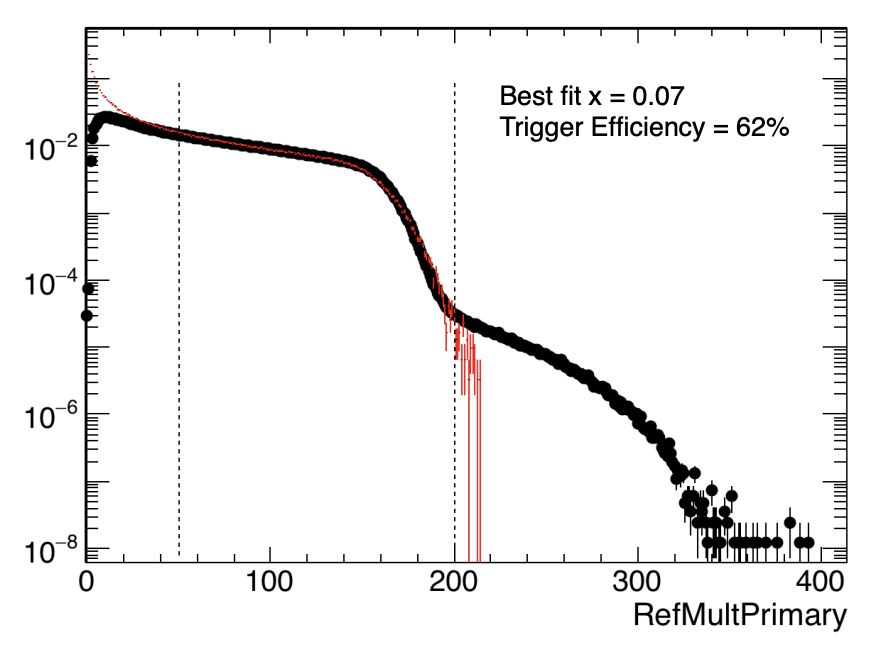
\includegraphics[scale=0.5]{FXT3gev/chapter1/fig/glauber_fit_ref.jpg}
    \caption{Uncorrected refmult distribution measured in the TPC within $|\eta|$ $<$ 0.5 in Au+Au collision at $\sqrt{s_{NN}}$=3GeV. The red line is the fit from Glauber Monte Carlo simulation.}
    \label{fig:glauber_fit}
\end{figure}

\begin{table}[h]
    \centering
    \begin{tabular}{c|c}
    \hline
        centrality & Refmult cut ($>$) \\
        \hline
        0-5\% &  133 \\ 
        5-10\% & 110 \\
        10-15\% & 92 \\
        15-20\% & 76 \\
        20-25\% & 63 \\
        25-30\% & 51 \\
        30-35\% & 42 \\
        35-40\% & 34 \\ 
        40-45\% & 27 \\
        45-50\% & 21 \\
        50-55\% & 16 \\
        55-60\% & 12 \\
        60-65\% & 9 \\
        65-70\% & 6 \\
        70-75\% & 4 \\
        75-80\% & 3 \\
        \hline
    \end{tabular}
    \caption{Refmult cut for centrality definition}
    \label{tab:cent_def}
\end{table}


